%%PREAMBLE %%%%%%%%%%%%%%%%%%%%%%%%%%%%
\documentclass[10pt, a4paper]{article}% size of txt = 10pt
\usepackage[top= 2cm,
			bottom = 2cm,
			left = 1.7cm,
			right = 1.7cm,
			footskip = 0.5cm,
			headsep = 0cm,
			headheight = 0cm
					]{geometry}
\usepackage{amsmath} % math packages
\usepackage{amsfonts}% math packages
\usepackage{amssymb} % math packages
\usepackage{graphicx} %package for including graphics
\usepackage{array}
\usepackage[thinlines]{easytable}
\usepackage{float}
\usepackage[section]{placeins}
\usepackage[hidelinks]{hyperref}
\usepackage[shortlabels]{enumitem}
\usepackage{svg}
\usepackage{bigstrut}
\usepackage{wrapfig,lipsum,booktabs}
\usepackage{subcaption}
\usepackage{xfrac}
\usepackage{pdfpages}
\usepackage{listings}
\usepackage{xcolor}
\usepackage{enumitem}

\usepackage{listings}
\usepackage{color} %red, green, blue, yellow, cyan, magenta, black, white
\definecolor{mygreen}{RGB}{28,172,0} % color values Red, Green, Blue
\definecolor{mylilas}{RGB}{170,55,241}

\definecolor{codegreen}{rgb}{0,0.6,0}
\definecolor{codegray}{rgb}{0.5,0.5,0.5}
\definecolor{codepurple}{rgb}{0.58,0,0.82}
\definecolor{backcolour}{rgb}{1,1,1}

\lstdefinestyle{mystyle}{
    backgroundcolor=\color{backcolour},   
    commentstyle=\color{codegreen},
    keywordstyle=\color{magenta},
    numberstyle=\tiny\color{codegray},
    stringstyle=\color{codepurple},
    basicstyle=\ttfamily\footnotesize,
    breakatwhitespace=false,         
    breaklines=true,                 
    captionpos=b,                    
    keepspaces=true,                 
    numbers=left,                    
    numbersep=5pt,                  
    showspaces=false,                
    showstringspaces=false,
    showtabs=false,                  
    tabsize=2
}
\lstset{style=mystyle}


%date format
\def\mydate{\leavevmode\hbox{\twodigits\day.\twodigits\month.\the\year}}
\def\twodigits#1{\ifnum#1<10 0\fi\the#1}

\usepackage{indentfirst}
\setlength{\parindent}{1cm}

\makeatletter
\newcommand{\thickhline}{%
    \noalign {\ifnum 0=`}\fi \hrule height 2pt
    \futurelet \reserved@a \@xhline
}
\newcolumntype{"}{@{\hskip\tabcolsep\vrule width 2pt\hskip\tabcolsep}}
\makeatother
\newcolumntype{?}{!{\vrule width 2pt}}
%%DOC ENVIROMENT%%%%%%%%%%%%%%%%%%%%%%%
\begin{document}
%Title 
\begin{flushleft}%% left justification
	\textbf{\Large{MKC-NBS: Úkol č. 2}}\hfill Filip Paul\\
	\large{Linková vrstva \hfill\mydate}
\end{flushleft}
\section*{\large{\textbf{Rámec Ethernet II:}}}
	\begin{itemize}[label={}]
		\item \textbf{Zadání:}\\
		Níže jsou uvedeny bajty dvou rámců typu Ethernet II, tak jak byly zachyceny programem 
		Wireshark. Tento program ve svých výpisech neuvádí návěští rámců ani jejich kontrolní součet, 
		takže tato pole v zadání nehledejte.\\

		\begin{minipage}{0.49\textwidth}
			\textbf{1. rámec:}\\
			01 00 5e 00 00 12 00 00 5e 00 01 01 08 00 45 c0\\
			00 28 00 00 00 00 ff 70 17 f0 c0 a8 01 fb e0 00\\
			00 12 21 01 c8 01 00 01 54 55 c0 a8 01 fe 00 00\\
			00 00 00 00 00 00 00 00 00 00 00 00
		\end{minipage}
		\begin{minipage}{0.49\textwidth}
			\textbf{2. rámec:}\\
			ff ff ff ff ff ff f0 f3 36 af f4 54 08 06 00 01\\ 
			08 00 06 04 00 01 00 07 0d af f4 54 18 a6 ac 01\\ 
			00 00 00 00 00 00 18 a6 ad 9f 06 01 04 00 00 00\\ 
			00 02 01 00 03 02 00 00 05 01 03 01
		\end{minipage}\\

		Z uvedených údajů zjistěte pro oba rámce cílovou a zdrojovou adresu a zjištěné adresy 
		charakterizujte (globální - skupinová - individuální, globální správa adresy - lokální správa adresy, 
		případně uveďte výrobce karty). Dále určete protokol, jehož zpráva je v těle daného rámce 
		přenášena. Potřebné informace lze získat například na následujících stránkách: 
		\href{https://www.iana.org/assignments/ethernet-numbers/ethernet-numbers.xhtml}{\color{blue} iana.org}
		a \href{https://www.adminsub.net/mac-address-finder}{\color{blue} adminsub.net}.

		\item \textbf{Vypracování:}\\
		Na následujícím obrázku je znázorněn postup "dekódování 1.rámce. Dekódování obou rámců bylo následně
		provedeno pomocí python scriptu, který nalzenete v příloze na konci dokumentu. Souhrnné
		výsledky pro první i druhý rámec a popis jednotlivých adres je na následující straně.
		\begin{figure}[ht!]
			\centering
			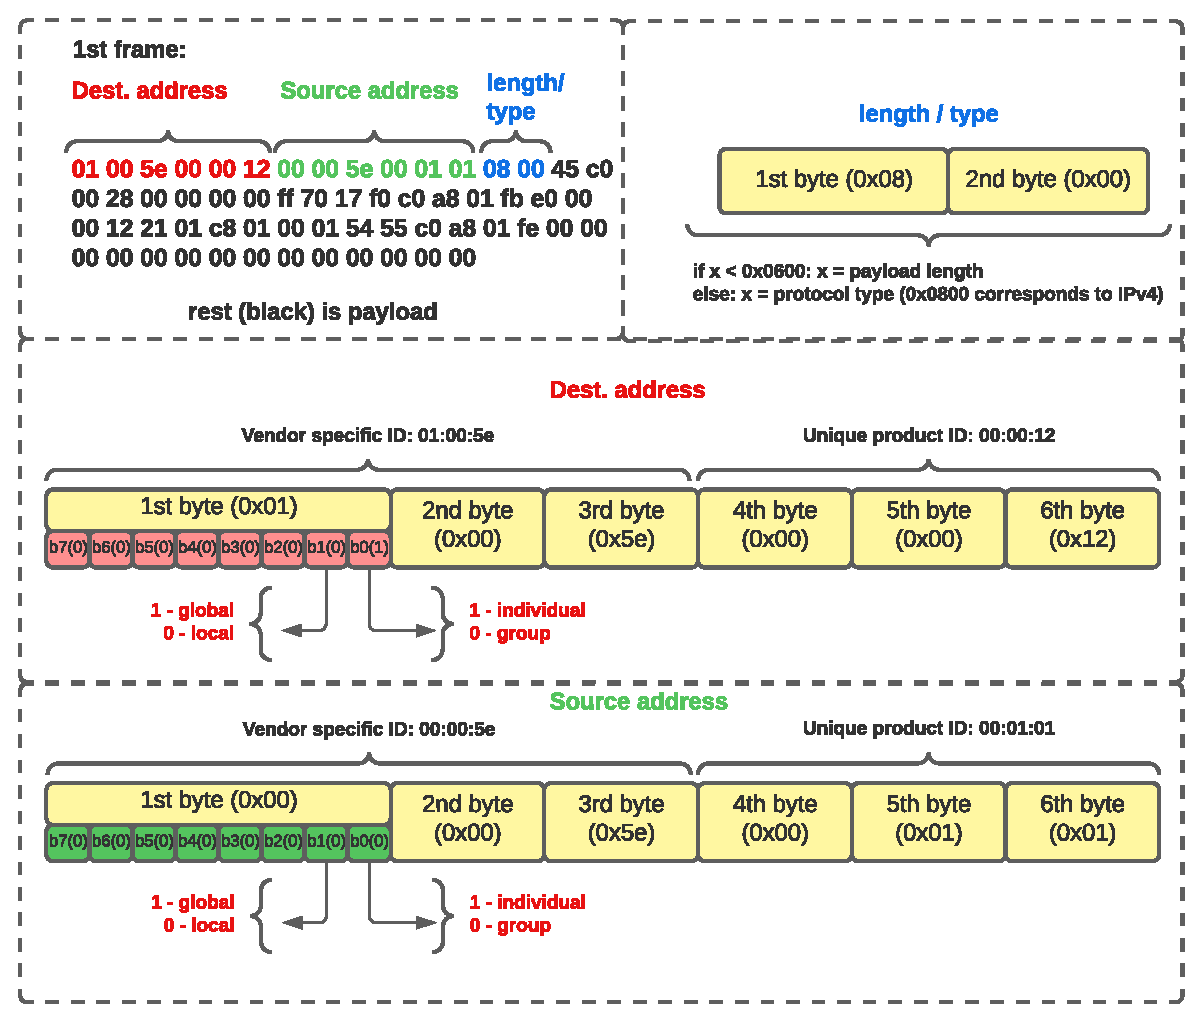
\includegraphics[width = 0.85\textwidth]{ethernet.eps}
		\end{figure}
		\clearpage

		\item \textbf{Popis jednotlivých typů adres:}
		\begin{itemize}[label=$\bullet$]
			\item \textbf{Globální (univerzální) vs lokální MAC adresa:}\\
			Globální MAC adresy jsou celosvětově unikátními identifikátory, které zařízením přidělují přímo jejich výrobci.
			Unikátnost není sice garantována, nicméně kolize dvou globálních MAC adres jsou velice nepravděpodobné.
			Lokální adresy jsou většinou přidělovány softwarem síťové karty a umožňují tak přepsat globální adresu. Zda je adresa
			lokální nebo globální lze rozlišit pomocí tzv. U/L bitu (viz obrázek na předchozí stránce).

			\item \textbf{Individuální (Unicast) vs skupinová (multicast) MAC adresa:}\\
			Individuální adresy mohou být jak zdrojové tak i cílové. Individuální adresa je určena pouze pro jedno zařízení
			s danou MAC adresou. Pokud cílové zařízení obrdží zprávu s individuální MAC adresou, která mu nenáleží, tak
			zprávu (frame) zignoruje.\\
			Skupinové adresy jsou pouze cílové. Zprávy, které mají skupinovou MAC adresu, jsou určené více zařízením zároveň.
			Speciálním typem je pak skupinová adresa s hodnotou FF:FF:FF:FF:FF:FF (Broadcast). Na zprávu s touto MAC adresou
			"slyší" všechny síťové karty. Boradcast se používa například při ARP. 
		\end{itemize}

			\textbf{Dekódování prvního rámce:}\\
			Destination address:\\
			first byte: 0x01 $\rightarrow$ 0b00000001 $\rightarrow$group and global adress.\\
			MAC: 01:00:5E:00:00:12 $\rightarrow$ Skupinová adresa pravděpodobně od výrobce ICANN, IANA Department\\\\
			Source address:\\
			first byte: 0x00 $\rightarrow$ 0b00000000 $\rightarrow$individual and global adress.\\
			MAC: 00:00:5E:00:01:01 $\rightarrow$ Vendor specific part: 00:00:5E ICANN, IANA Department\\\\
			lengt/type:\\
			0x0800 $\rightarrow$ DEC: Value is bigger than DEC: 1536 $\rightarrow$ Ethertype is: IPv4\\
			
			\textbf{Dekódování druhého rámce:}\\
			Destination address:\\
			first byte: 0xFF $\rightarrow$ 0b11111111 $\rightarrow$ Broadcast.\\
			MAC: FF:FF:FF:FF:FF:FF $\rightarrow$ Broadcast\\\\
			Source address:\\
			first byte: 0xF0 $\rightarrow$ 0b11110000 $\rightarrow$individual and global adress.\\
			MAC: F0:F3:36:AF:F4:54 $\rightarrow$ Vendor specific part: F0:F3:36 TP-LINK TECHNOLOGIES CO.,LTD.\\\\
			lengt/type:\\
			0x0806 $\rightarrow$ DEC: Value is bigger than DEC: 1536 $\rightarrow$ Ethertype is: ARP
		\end{itemize}
	
	\clearpage
	\section*{\large{\textbf{ Protokol STP:}}}
		\begin{itemize}[label={}]
			\item \textbf{Zadání:}\\
			Je dána ethernetová síť sestávající ze čtyř přepínačů s identifikátory 1, 2, 3 a 4. Tyto přepínače jsou 
			propojeny podle níže uvedeného obrázku. Pro zadanou síť určete pomocí algoritmu STP její kostru. 
			Přenesené zprávy zapište do přehledné tabulky a zjištěnou kostru zakreslete s vyznačením, které porty jsou zapnuty a které blokovány.

			\item \textbf{Vypracování:}\\
			\begin{figure}[ht!]
				\centering
				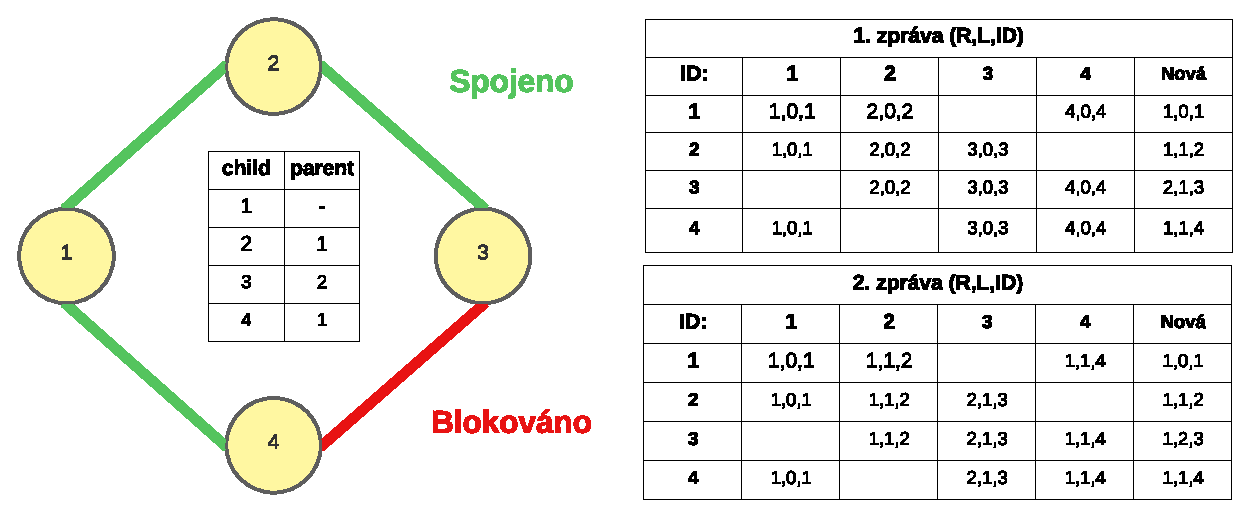
\includegraphics[width = 0.9\textwidth]{STP.eps}
			\end{figure}
		\end{itemize}

	\clearpage
	\section*{\large{\textbf{Přílohy:}}}

	\begin{itemize}[label={}]
		\item \textbf{EthernetFrame.py}\\
		\lstinputlisting[language=python]{calc.py}
		\clearpage
	\end{itemize}

\end{document}